\documentclass[tikz,border=8pt]{standalone}
\begin{document}
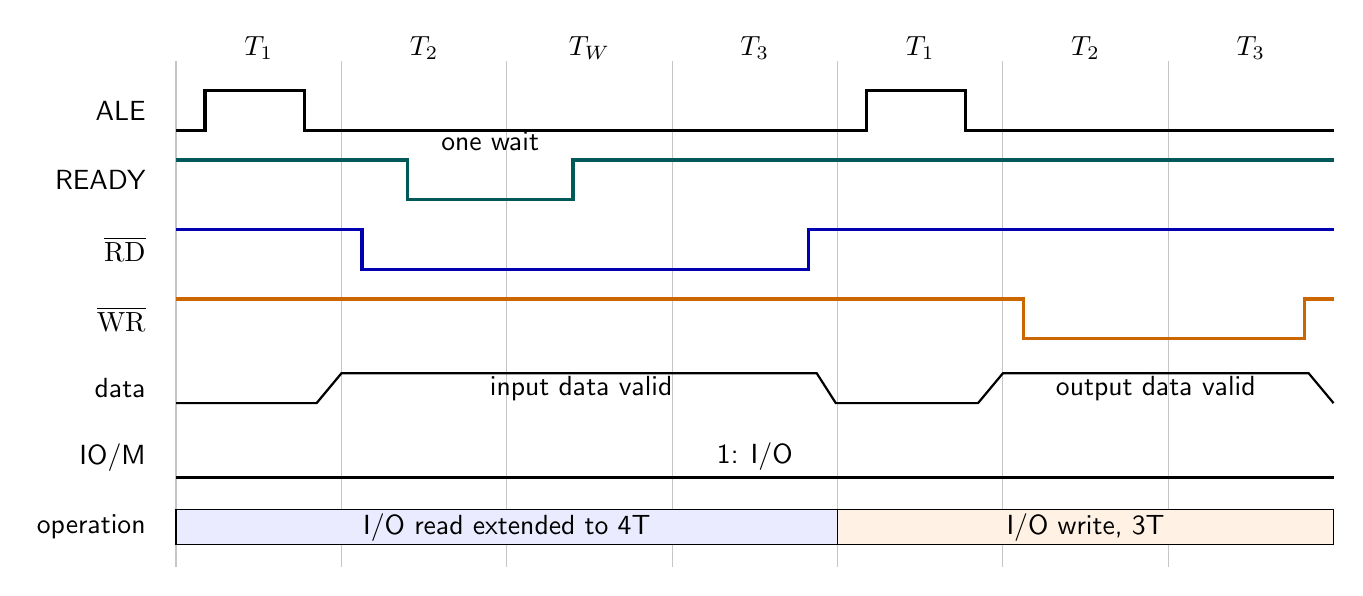
\begin{tikzpicture}[font=\sffamily,x=1.05cm,y=.63cm]
\foreach \x/\t in {0/$T_1$,2/$T_2$,4/$T_W$,6/$T_3$,8/$T_1$,10/$T_2$,12/$T_3$}{\draw[gray!45] (\x,-.1)--(\x,10.1);\node at (\x+1,10.35){\t};}
\node[anchor=east] at (-.25,9.1){ALE};\node[anchor=east] at (-.25,7.7){READY};\node[anchor=east] at (-.25,6.3){$\overline{\rm RD}$};\node[anchor=east] at (-.25,4.9){$\overline{\rm WR}$};\node[anchor=east] at (-.25,3.5){data};\node[anchor=east] at (-.25,2.1){IO/M};\node[anchor=east] at (-.25,.7){operation};
\draw[very thick] (0,8.7)--(.35,8.7)--(.35,9.5)--(1.55,9.5)--(1.55,8.7)--(8.35,8.7)--(8.35,9.5)--(9.55,9.5)--(9.55,8.7)--(14,8.7);
\draw[very thick,teal!70!black] (0,8.1)--(2.8,8.1)--(2.8,7.3)--(4.8,7.3)--(4.8,8.1)--(14,8.1);\node[above] at (3.8,8.1){one wait};
\draw[very thick,blue!70!black] (0,6.7)--(2.25,6.7)--(2.25,5.9)--(7.65,5.9)--(7.65,6.7)--(14,6.7);
\draw[very thick,orange!80!black] (0,5.3)--(10.25,5.3)--(10.25,4.5)--(13.65,4.5)--(13.65,5.3)--(14,5.3);
\draw[thick] (0,3.2)--(1.7,3.2)--(2,3.8)--(7.75,3.8)--(7.98,3.2)--(9.7,3.2)--(10,3.8)--(13.7,3.8)--(14,3.2);
\node at (4.9,3.5){input data valid};\node at (11.85,3.5){output data valid};
\draw[very thick] (0,1.7)--(14,1.7);\node at (7,2.12){1: I/O};
\draw[fill=blue!8] (0,.35) rectangle (8,1.05);\node at (4,.7){I/O read extended to 4T};\draw[fill=orange!10] (8,.35) rectangle (14,1.05);\node at (11,.7){I/O write, 3T};
\end{tikzpicture}
\end{document}
